\documentclass[11.5pt]{sig-alternate} % sets document style to sig-alternate
% packages
% typesetting
%\usepackage{dirtytalk} % typset quotations easier (\say{stuff})
\usepackage{hanging} % hanging paragraphs
\usepackage[defaultlines=3,all]{nowidow} % avoid widows
\usepackage[pdfpagelabels=false]{hyperref} % produce hypertext links, includes backref and nameref
\usepackage{xurl} % defines url linebreaks, loads url package
\usepackage{microtype}
\usepackage{textgreek}
%\usepackage{textcomp}
%\newcommand{\texttildemid}{\raisebox{0.4ex}{\texttildelow}}
\usepackage{amsmath}
% layout
\usepackage{enumitem} % control layout of itemize, enumerate, description
\usepackage{fancyhdr} % control page headers and footers
\usepackage{float} % improved interface for floating objects
%\usepackage{multicol} % intermix single and multiple column pages
% language
\usepackage[utf8]{inputenc} % accept different input encodings
\usepackage[english]{babel} % multilanguage support
% misc
\usepackage{graphicx} % builds upon graphics package, \includegraphics
%\usepackage{lastpage} % reference number of pages
%\usepackage{comment} % exclude portions of text (?)
\usepackage{xcolor} % color extensions
\usepackage[backend=biber, style=apa]{biblatex} % sophisticated bibliographies % necessary for HTML to display author info and date on abstract page
\usepackage{csquotes} % advanced quotations, makes biblatex happy
\usepackage{authblk} % support for footnote style author/affiliation
% tables and figures
\usepackage{tabularray}
\usepackage{circledsteps}
%\usepackage{array} % extend array and tabular environments
\usepackage{caption} % customize captions in figures and tables (rotating captions, sideways captions, etc)
%\usepackage{cuted} % allow mixing of \onecolumn and \twocolumn on same page
\usepackage{multirow} % create tabular cells spanning multiple rows
%\usepackage{subfigure} % deprecated, support for manipulation of small figures
%\usepackage{tabularx} % extension of tabular with column designator "x", creates paragraph-like column whose width automatically expands
%\usepackage{wrapfig} % allows figures or tables to have text wrapped around them
%\usepackage{booktabs} % better rules
% dummy text
%\usepackage{blindtext} % blind text dummy text
%\usepackage{kantlipsum} % Kant style dummy text
\usepackage{lipsum} %lorem ipsum dummy text
% other helpful packages may be booktabs, longtable, longtabu, microtype

\pagestyle{fancy} % sets pagestyle to fancy for fancy headers and footers

% header and footer
% modern way to set header image
\renewcommand{\headrulewidth}{0pt} % defines thickness of line under header
\renewcommand{\footrulewidth}{0pt} % defines thickness of line above header
\setlength\headheight{80.0pt} % sets height between top margin and header image, effectively moves page contents down
\addtolength{\textheight}{-80.0pt} % seems to affect the lower height. maybe only works properly if footer numbers enabled?
\fancyhf{}
\fancyhead[CE, CO]{
\includegraphics[width=\textwidth]{headerImage.png}}
% footer
%\fancyfoot[LE,LO]{Article Title Here \\ DOI: }% left footer article title and doi
%\fancyfoot[CE,CO]{{}} % center footer empty
%\fancyfoot[RE,RO]{\thepage} % right footer page numbers
%\pagenumbering{arabic} % arabic (1, 2, 3) numbering in footer

\hypersetup{colorlinks=true,urlcolor=blue} % sets link color to blue
\urlstyle{same} % sets url typeface to same as rest of text

% set caption and figure to italics, label bold, left align captions, does not transfer to HTML
\captionsetup{labelfont=bf, font={large, it}, justification=raggedright, singlelinecheck=false}
\renewcommand\theContinuedFloat{\alph{ContinuedFloat}}

%this next bit is confusing, but essentially changes the width of the abstract. Seems to have been copied from this https://tex.stackexchange.com/questions/151583/how-to-adjust-the-width-of-abstract
\let\oldabstract\abstract
\let\oldendabstract\endabstract
\makeatletter %changes @ catcode to enable modification (in parsep)
\renewenvironment{abstract} %alters the abstract environment
{\renewenvironment{quotation}%
               {\list{}{\addtolength{\leftmargin}{1em} % change this value to add or remove length to the the default ?
                        \listparindent 1.5em%
                        \itemindent    \listparindent%
                        \rightmargin   \leftmargin%
                        \parsep        \z@ \@plus\p@}%
                \item\relax}%
               {\endlist}%
\oldabstract}
{\oldendabstract}
\makeatother %changes @ catcode to disable modification



% checks
% italics
% links
% dashes
% tildes
\begin{document}

\title{Solving Word Problems: As Easy as PIES!}

\author[1]{\large \color{blue}Mary Jane Heater}
\author[2]{\large \color{blue}Lori A. Howard}
\author[3]{\large \color{blue}Ed Linz}

\affil[1]{Fairfax County Public Schools}
\affil[2]{University of Virginia}
\affil[3]{. Educational Consultant}

\toappear{}
%% ABSTRACT
\maketitle
\begin{@twocolumnfalse} 
\begin{abstract}
\item 
\textit{Many students are challenged when tasked to complete a word problem.  While they may know the procedural steps to solve an equation, translating a word problem into an appropriate equation and producing a solution may often cause students to become confused or unwilling to try.  This article provides a potential solution for teachers by discussing the use of a simple mnemonic tool to help organize the process.  Mnemonics are a useful and effective strategy to help students with learning disabilities remember information and process steps.  In the strategy presented, the mnemonic \textbf{PIES} is used to describe a 4-step process for solving word problems in which the acronym is described as \textbf{P}=Picture (draw a simple sketch) based on the situation described by the word problem), \textbf{I}=Information (circle key words in the problem and write next to picture), \textbf{E}=Equation (find an equation that fits the information), and \textbf{S}=Solve (solve the equation to produce an answer). \textbf{PIES} has been successfully used with all students in an inclusive high school Physics classroom, as well as self-contained high school science classes. Suggestions and an example for teachers are included.}
\\ \\
 
\end{abstract}
\end{@twocolumnfalse}

%% AUTHOR INFORMATION

\textbf{*Corresponding Author, Mary Jane Heater}\\
\href{mailto: mjheater@ymail.com }{(mjheater@ymail.com)} \\
\textit{Submitted Dec 18 2013 }\\
\textit{Accepted Dec 18 2013} \\
\textit{Published online Dec 18 2013 } \\
\textit{DOI:10.14448/jsesd.05.0002} \\
\pagebreak
\clearpage

\begin{large}
    
Developing effective student problem solving skills to present to students has been an ongoing challenge for educators.  For a variety of reasons, the challenge is magnified for students with learning disabilities (Mastropieri \& Scruggs, 2010).  Some students, for example, may have difficulties in organization, while others experience reading comprehension issues.  In this article, we present an effective mnemonic that has produced improvement in performance for students of all skill levels in our classroom, particularly those students with learning disabilities. This mnemonic strategy has been successfully used in our inclusive high school Physics classroom, as well as self-contained high school science classes.  Additionally, the Algebra 1 teacher reports that students co-enrolled in inclusive Physics and Algebra 1 have also shown improvement in their ability to solve word problems in the Mathematics class.

How many times have teachers heard students proclaim, "I can't do word problems!"?   This student refrain is often genuine, based on years of frustration and failure, particularly for students challenged by learning disabilities. Although many students have the ability to solve basic STEM (Science, Technology, Engineering, and Mathematics) equations, such as 10 + 2 x = 20, they immediately shut down when presented with the following word problem:   

\textbf{Carla is driving at 10 m/s when she speeds up (accelerates) at 2 m/s\textsuperscript{2}. If her new speed is now 20 m/s, how long was she accelerating?}

It turns out that the initial equation, 10 + 2 x = 20 will provide the solution to the word problem.  But for a vast number of students, the verbal aspects of the word problem pose what they perceive to be as an insurmountable problem.  They simply do not know where, or how, to begin.  A frequent response for many students is to skip this problem, or if attempting a multiple choice assessment, to immediately guess one of the given answers and move on to the next question.   

Our approach is to break this cycle of despair by providing students with a methodology with which to begin and a simple, standard approach which leads the student through a process leading to correct solutions.  This series of easy-to-follow-steps can be used by every student in the inclusive science classroom (Linz, Heater, \& Howard, 2011). Our classroom experience is that the mnemonic \textbf{PIES} is quickly learned and can be applied to a variety of word problems from introductory Physics through Advanced Placement (AP) courses.

This approach uses a mnemonic to help students learn and remember the steps needed for solving word problems. The use of mnemonics is an effective strategy for helping all students, but has been shown to be particularly effective for students with disabilities (Forness, Kavale, Blum, \& Lloyd, 1997). In addition, mnemonics have been found to be useful in teaching science content to students with learning disabilities (Therrien, Taylor, Hosp, Kaldenberg, \& Gorsh, 2011). You may already be familiar with the acrostic \textbf{K}ing \textbf{P}hilip \textbf{C}ame \textbf{O}ver \textbf{F}or \textbf{G}reen \textbf{S}oup used in a Biology class to assist students learning Kingdom, Phylum, Class, Order, Family, Genus, Species. Or, you may use the acronym \textbf{PEN} for Protons, Electrons and Neutrons.  Simply put, many teachers are frequent users of acronyms to assist student learning.  Our suggested approach for solving word problems uses a very easy-to-remember acronym. 

We call the process \textbf{PIES}. The acronym stands for

\textbf{Picture} - draw a simple \textbf{\textit{picture}} showing the situation

\textbf{Information} - find important facts (\textbf{\textit{information}}) and list them next to the picture

\textbf{Equation} - find an \textbf{\textit{equation}} which match the information on the picture

\textbf{Solve} - insert information from picture into equation and \textbf{\textit{solve}} algebraically

Let's apply the \textbf{PIES} process to the beginning Physics motion problem described above.  The first step for the student is to read the entire problem and to gather sufficient information to draw a rough \textbf{\textit{Picture}}, or sketch, of the situation described by the words.  Stick figures work great.  The idea is to get the students \textit{started}.  No longer are they simply staring at words; they have now done what many simply cannot do - they have started solving a word problem.  Here is an acceptable picture:

\begin{figure}[h]
    \centering
    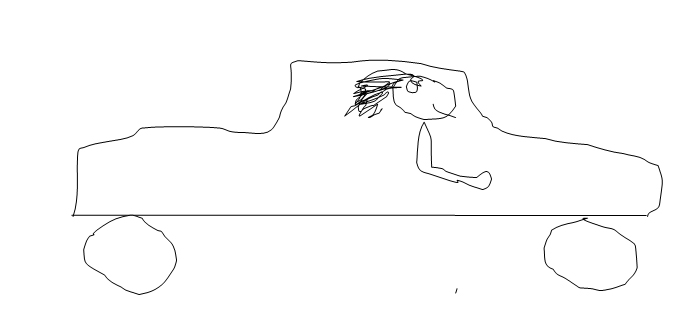
\includegraphics[width=1\linewidth]{img1.jpg}
\end{figure}

Although this sketch will probably not win an art award, it does serve the purpose of having the student \textit{get started} on the word problem.  The student is no longer staring at the words, but is now actively involved in the process of solving the problem.  This is the \textit{\textbf{P}icture} part of \textbf{PIES}.  When assessing student work, we give partial credit for this sketch (e.g., 2 of the 10 points for the entire problem), even if that is all the student is able to do.  Our rationale is that the student has become engaged in the problem solving process – a particularly significant progress marker for the student who has a history of not even attempting such problems. As the student continues the \textbf{PIES} process, additional points are awarded for each successful completion of parts of the problem.  The incremental awarding of points provides reinforcement in motivating students to continue working through the process (Mastropieri \& Scruggs, 2010)

The next step is for the student to “mine” the word problem to find important \textbf{\textit{Information}} which can be added to the picture which has been drawn.  Although we initially use the word “mine” to describe the process to the students, we also include follow on descriptors for their actions, such as “find” and “discover” or “dig out.”  To do this excavation, we select students whom we know to be comfortable reading aloud to start to read the word problem.  We simultaneously challenge the entire class to yell “STOP” when the reader reaches a piece of information which is deemed to be important.  Our goal is to have the entire class involved.  Another option which we have used is to have one student designated to read, and another to yell STOP.  

As the designated student begins to read the given problem, “\textbf{Carla is driving at 10 m/s}.” Ask students the following questions:
\begin{enumerate}
    \item “Why did you yell STOP?”
    \item “Is that an important piece of information?”
    \item “What type of information is 10 m/s?”
\end{enumerate}

Sometimes we select a different student and ask the same questions.  The purpose is to identify that 10 m/s is definitely important information and to continue questioning until it is correctly identified as the speed or the velocity, which we call “\textbf{v.}”  We then tell all the students to circle that information (as shown below).

\textbf{Carla is driving \CircledText{at 10 m/s}}

and to then \textbf{add} that information to the picture which they have drawn.

\[v = 10\;m/s\]

\begin{figure}[h]
    \centering
    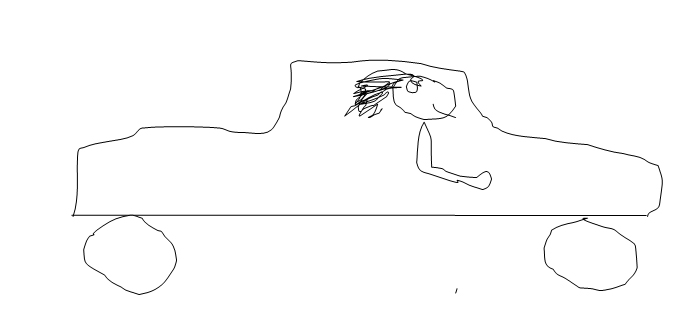
\includegraphics[width=0.95\linewidth]{img1.jpg}
\end{figure}

The student is now in the second step of the \textbf{PIES} process, that is, finding and applying \textit{\textbf{I}nformation} to the \textit{\textbf{P}icture}. Another student is selected to continue reading aloud until the next piece of important information is discovered

\textbf{ …… when she speeds up (accelerates) at 2 m/s\textsuperscript{2}.}

Most students are told to stop either at “speeds up” or “at \textbf{2 m/s\textsuperscript{2}}.”   We then quiz the class as to what acceleration means, have them circle this new important information, and add it to the diagram.  We now have 

\textbf{Carla is driving \CircledText{at 10 m/s} when she speeds up \CircledText{(accelerates) at 2 m/s\textsuperscript{2}.}}

and 
\begin{align*}
    v &= 10\;m/s \\
    a &= 2\;m/s^{2}
\end{align*}
\begin{figure}[h]
    \centering
    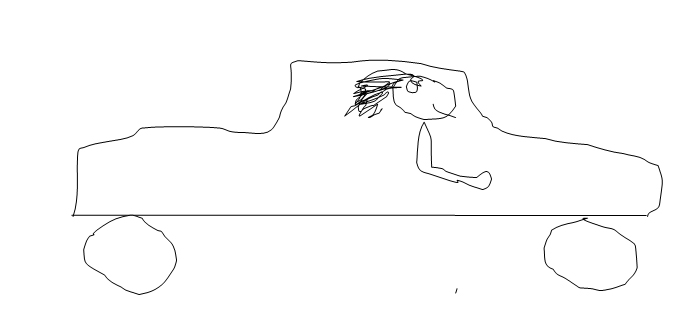
\includegraphics[width=0.95\linewidth]{img1.jpg}
\end{figure}

We continue the \textit{\textbf{I}nformation} mining process with another student who reads aloud and finds “\textbf{new speed is 20 m/s}.”  This piece of information provides an opportunity for a more advanced inquiry because we now have two pieces of speed or velocity information.  “Which type or name of speed is this new one, the 20 m/s?” we ask.  “Is that the initial speed or the final speed?”  Often other students will volunteer the correct answer quickly, that is, the \textbf{\textit{final}} speed.  So after circling this latest information mined from the word problem, the students are directed to not only add \textbf{v\textsubscript{f}  = 20 m/s} to their picture, but to add a subscript i to the previous speed information to distinguish it from the final speed.  We now have:

\textbf{Carla is driving \CircledText{at 10 m/s} when she speeds up \CircledText{(accelerates) at 2 m/s\textsuperscript{2}.} If her new speed is \CircledText{20 m/s}.....}

and the picture now becomes
\begin{align*}
    v_{i} &= 10\;m/s \\
    a &= 2\;m/s^{2} \\
    v_{f} &= 20\;m/s
\end{align*}
\begin{figure}[h]
    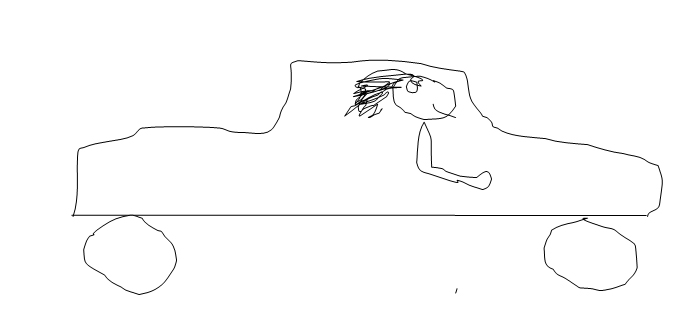
\includegraphics[width=1\linewidth]{img1.jpg}
\end{figure}

But the student is not finished.  There are more words left in the problem, and they are just as important as the others.  We often read the final words to the student:

“\textbf{How long was she accelerating?}” So what is it that we are trying to find?...there are often several answers, but ultimately a majority of the students settle on \textbf{time, t}. 

It is important to stress to the students that this final quantity is just as important as the other information, and that it MUST be added to the picture.  Because there is no numerical figure associated with this quantity, we still must write it down, so that we have ALL the information.  Since we do not know its value yet, we will label it with a question mark.  Our word problem has now been completely mined.

\textbf{Carla is driving \CircledText{at 10 m/s} when she speeds up \CircledText{(accelerates) at 2 m/s\textsuperscript{2}.} If her new speed is now \CircledText{20 m/s,} \CircledText{how long} was she accelerating?}

and our completed picture is now:
\begin{align*}
    v_{i} &= 10\;m/s \\
    a &= 2\;m/s^{2} \\
    v_{f} &=20\;m/s \\
    t &= ?
\end{align*}
\begin{figure}[h]
    \centering
    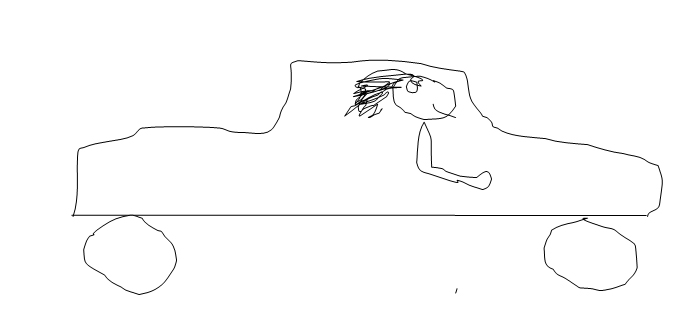
\includegraphics[width=1\linewidth]{img1.jpg}
\end{figure}

The students who have now successfully completed the \textbf{\textit{Information}} part of \textbf{PIES} are awarded additional partial credit (e.g., 2 more points out of the 10 assigned for this problem). We provide verbal encouragement by reminding students that they have now completed essentially 50\% of a word problem.

Students are now ready for the next step of \textbf{PIES}, finding the correct \textbf{\textit{Equation}} to use to solve the problem. We always provide a list of applicable equations, although some teachers may prefer not to do so. Our classroom experience is that students with learning disabilities benefit from having a “shopping list” of equations to choose from. We also  note that comparable lists are provided for students taking Advanced Placement examinations. Our goal with \textbf{PIES} is to teach a \textit{process} for solving problems, not to complicate the issue by forcing memorization of equations. The applicable numbered equation list (or “bank” – similar to word banks) provided with this “Carla” problem is:  
\begin{align}
    d &= v (t) \\
    d &= v_{i} (t) + \frac{1}{2} a (t^{2}) \\
    v_{f} &= v_{i} + a (t) \\
    v_{f}\vspace{1em}^{2} &= v_{i}\vspace{1em}^{2} + 2 (a) (d)
\end{align}
[We have found that the numbering of the equations is very helpful for students with learning disabilities.]

We now direct students to look at their picture and the information which they have written on it in order to locate one of the equations which has all 4 variables, that is, it must have a \textbf{v\textsubscript{i}}, \textbf{a}, \textbf{v\textsubscript{f}}, and \textbf{t} in it.  There is typically some initial confusion, but soon each student sees that only equation (3) contains the correct variables.  But the students are NOT finished with the \textbf{\textit{Equation}} part of with \textbf{PIES} until they write out the equation (legibly and accurately) under their picture.  At this point they are ¾ finished with the problem. Note that they do not yet have an answer, but they are now 75\% there. All that is left is to \textbf{\textit{Solve}} the chosen equation algebraically.  Again the students are rewarded with additional credit for this part of their work. Their work should now look like this:
\begin{align*}
    v_{i} &= 10\;m/s \\
    a &= 2\;m/s^{2} \\
    v_{f} &= 20\;m/s \\
    t &= ?
\end{align*}
\begin{figure}[!h]
    \centering
    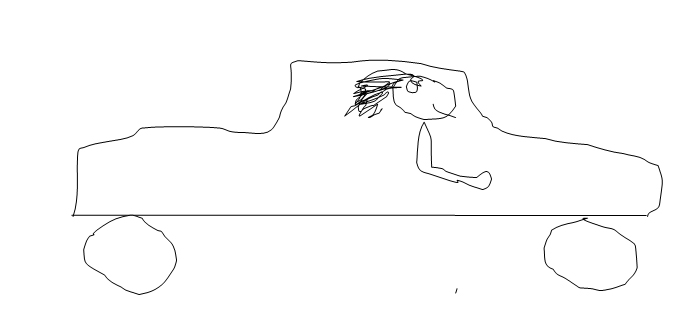
\includegraphics[width=1\linewidth]{img1.jpg}
\end{figure}
\[v_{f} = v_{i} + a (t)\]
Now the students are instructed to simply take the information which they placed on their picture in the correct location directly below the equation which they have placed below their picture. We do not include units (although some teachers may choose to do so).  Our classroom experience is that students with learning disabilities can be distracted by the presence of both unit and number in an equation, and that, so long as the MKS (meters, kilograms, seconds) units are being used, the correct unit for the answer will be apparent. Typical student work should look like this:
\begin{align*}
    v_{f} &= v_{i} + a (t) \\
    20 &= 10 + 2 (t) \\
    10 &= 2 (t) \\
    5 &= t
\end{align*}
Now we ask, “What are the correct MKS units for Time?”  Most (but not all) enthusiastically reply “Time” and are then directed to use their answers to complete the solution,  t  = 5  sec. But we are not finished until the student indicates that this is their answer to the problem by circling the answer,
\[\Circled{t = 5\;sec}\]
The entire \textbf{PIES} process now looks like this:

Carla is driving \CircledText{at 10 m/s} when she speeds up \CircledText{(accelerates) at 2 m/s\textsuperscript{2}.} If her new speed is now \CircledText{20 m/s,} \CircledText{how long} was she accelerating?
\begin{align*}
    v_{i} &= 10\;m/s \\
    a &= 2\;m/s^{2} \\
    v_{f} &= 20\;m/s \\
    t &= ?
\end{align*}
\begin{figure}[!h]
    \centering
    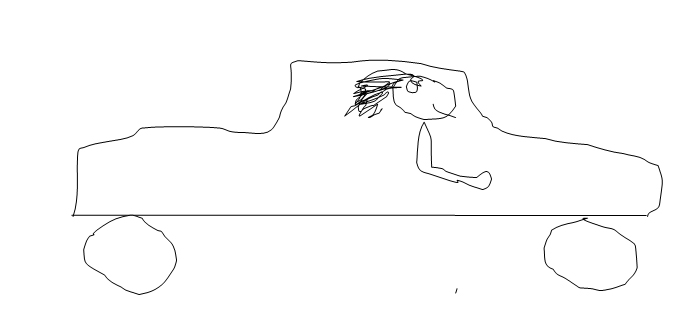
\includegraphics[width=1\linewidth]{img1.jpg}
\end{figure}
\begin{align*}
    v_{f} &= v_{i} + a (t) \\
    20 &= 10 + 2 (t) \\
    10 &= 2 (t) \\
    5 &= t
\end{align*}
\[\Circled{t = 5\;sec}\]

In terms of assessment, we can now award the student who has successfully completed the entire problem using the \textbf{PIES} process (including circling the answer) the full amount of points (e.g., 10 out of 10).  Once students become comfortable and proficient with \textbf{PIES}, they look forward to earning credit on an incremental basis rather than the “go-no go” grading associated with multiple-choice assessments. An additional benefit is that teachers are able to better analyze exactly where students are having difficulty in successfully completing word problems. Interestingly, we have found that the most common challenge for students is not completing the algebraic component, but in finding the appropriate equation to use.  Providing a process to determine the correct equation is one of the many benefits of \textbf{PIES}.

In conclusion, the acronym \textbf{PIES} used for remembering process steps and awarding of points for each step of the process has been successful in our inclusive high school Physics classroom and in self-contained science classroom for students with learning disabilities. \textit{All} students in our Physics classes, not just those with learning disabilities, use the mnemonic when solving word problems. We have also found that homework with assigned word problems is more complete when students apply \textbf{PIES}.  Students appear to gain confidence as evidenced by their attempts to complete all of the assigned homework problems. In the past, homework with assigned word problems would be incomplete as students would not attempt to solve the word problems or only provide answers without showing their work.  

Students are also encouraged to use \textbf{PIES} when taking tests in our class and on the end of the year standardized tests.  During unit tests, students are awarded points for each step of the process which also serves to reward students for making an attempt at each question. Although \textbf{PIES} was developed to assist students with learning disabilities in an inclusive high school Physics classroom, students in self-contained classes, as well as Algebra 1 classes have also used \textbf{PIES} successfully. It is a mnemonic for solving word problems that may benefit students in all science content areas and at other skill-levels, including Advanced Placement (AP) courses. 

\section*{BIOGRAPHICAL STATEMENTS}
\textbf{Mary Jane Heater} \href{mailto:mjheater@ymail.com}{(mjheater@ymail.com)}, Mary Jane Heater, a retired high school special education teacher, taught for 10 years at West Springfield High School, Springfield, Virginia. Classes she taught, as either the content or team teacher, include Biology, Algebra I, Physics, Personal/Financial Math. She graduated with a BA from The College of Wooster, and a M.Ed from The University of Virginia. Mrs. Heater currently resides in Canberra, Australia with her husband and two cats.

\textbf{Lori A. Howard} \href{mailto:howardl@marshall.edu}{(howardl@marshall.edu)}, Lori A. Howard, Ph.D. is an Assistant Professor of Special Education at Marshall University. She has taught a variety of special education courses. She has written and presented at conferences on the topics of inclusion, co-teaching, students with disabilities in science, and including students with disabilities in advanced placement courses.

\textbf{Ed Linz} \href{mailto:erlinz@fcps.edu}{(erlinz@fcps.edu)} Ed Linz, a retired commander of nuclear submarines, taught high school Physics and Mathematics for 27 years in public schools in Northern Virginia. He is a graduate of the U.S. Naval Academy and holds advanced degrees from Oxford University and George Mason University. Mr. Linz currently writes and lectures as an educational consultant.

\end{large}
\clearpage
\section*{REFERENCES}\par 

\leftskip 0.25in
\parindent -0.25in 
Forness, S. R., Kavale, K.A., Blum. I. M., \& Lloyd, J. W. (1997). Mega-analysis of meta-analyses: What works in special education and related services. \textit{TEACHING Exceptional Children, 29}(6) 4-9.

Linz, E., Heater, M. J., \& Howard, L.A. (2011). \textit{Team teaching science: Success for all learners}. Washington, D.C.: National Science Teachers Association.

Mastropieri, M.A, \& Scruggs, T.E., (2010). The Inclusive Classroom: \textit{Strategies for effective instruction (4th ed.)}. Upper Saddle River, NJ: Pearson.

Therrien, W. J., Taylor, J.C., Hosp, J.L., Kaldenberg, E.R., \& Gorsh, J. (2011). Science instruction for students with learning disabilities: A meta-analysis. \textit{Learning Disabilities Research \& Practice. 26}(4) 188-203.

\end{document}
